\documentclass[../AnalysisNoteJBuxton.tex]{subfiles}
\begin{document}

\section{Correlation Functions}
\label{CorrelationFunctions}

General remarks about formaton of correlation functions and what information they provide.

\begin{figure}[h]
  \centering
  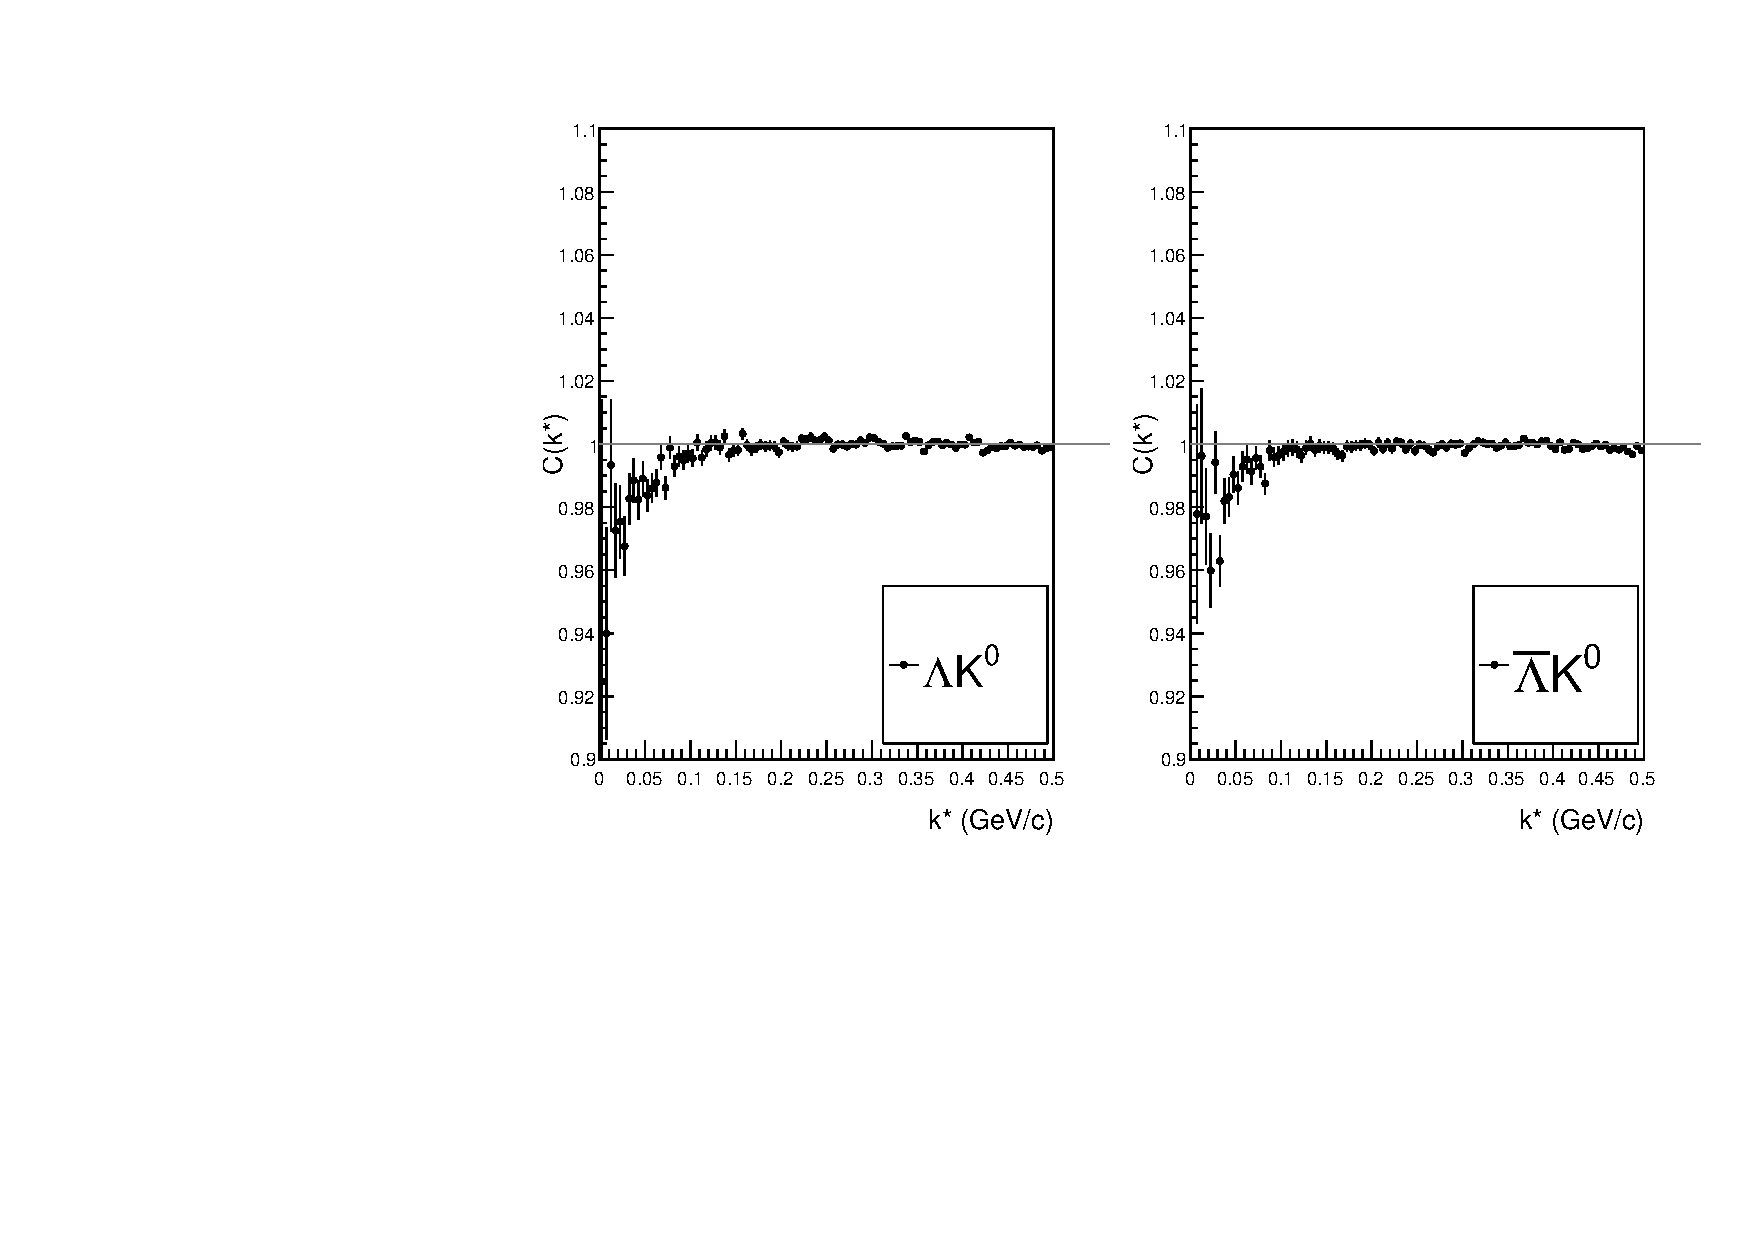
\includegraphics[width=\textwidth]{4_CorrelationFunctions/Figures/canKStarCfLamK0_0010.pdf}
  \caption[All $\Lambda$($\bar{\Lambda}$)K$^{0}_{S}$ Correlation Functions]{All $\Lambda$($\bar{\Lambda}$)K$^{0}_{S}$ Correlation Functions for 0-10\% Centrality}
  \label{fig:cLamK0Cfs0010}
\end{figure}

\begin{figure}[h]
  \centering
  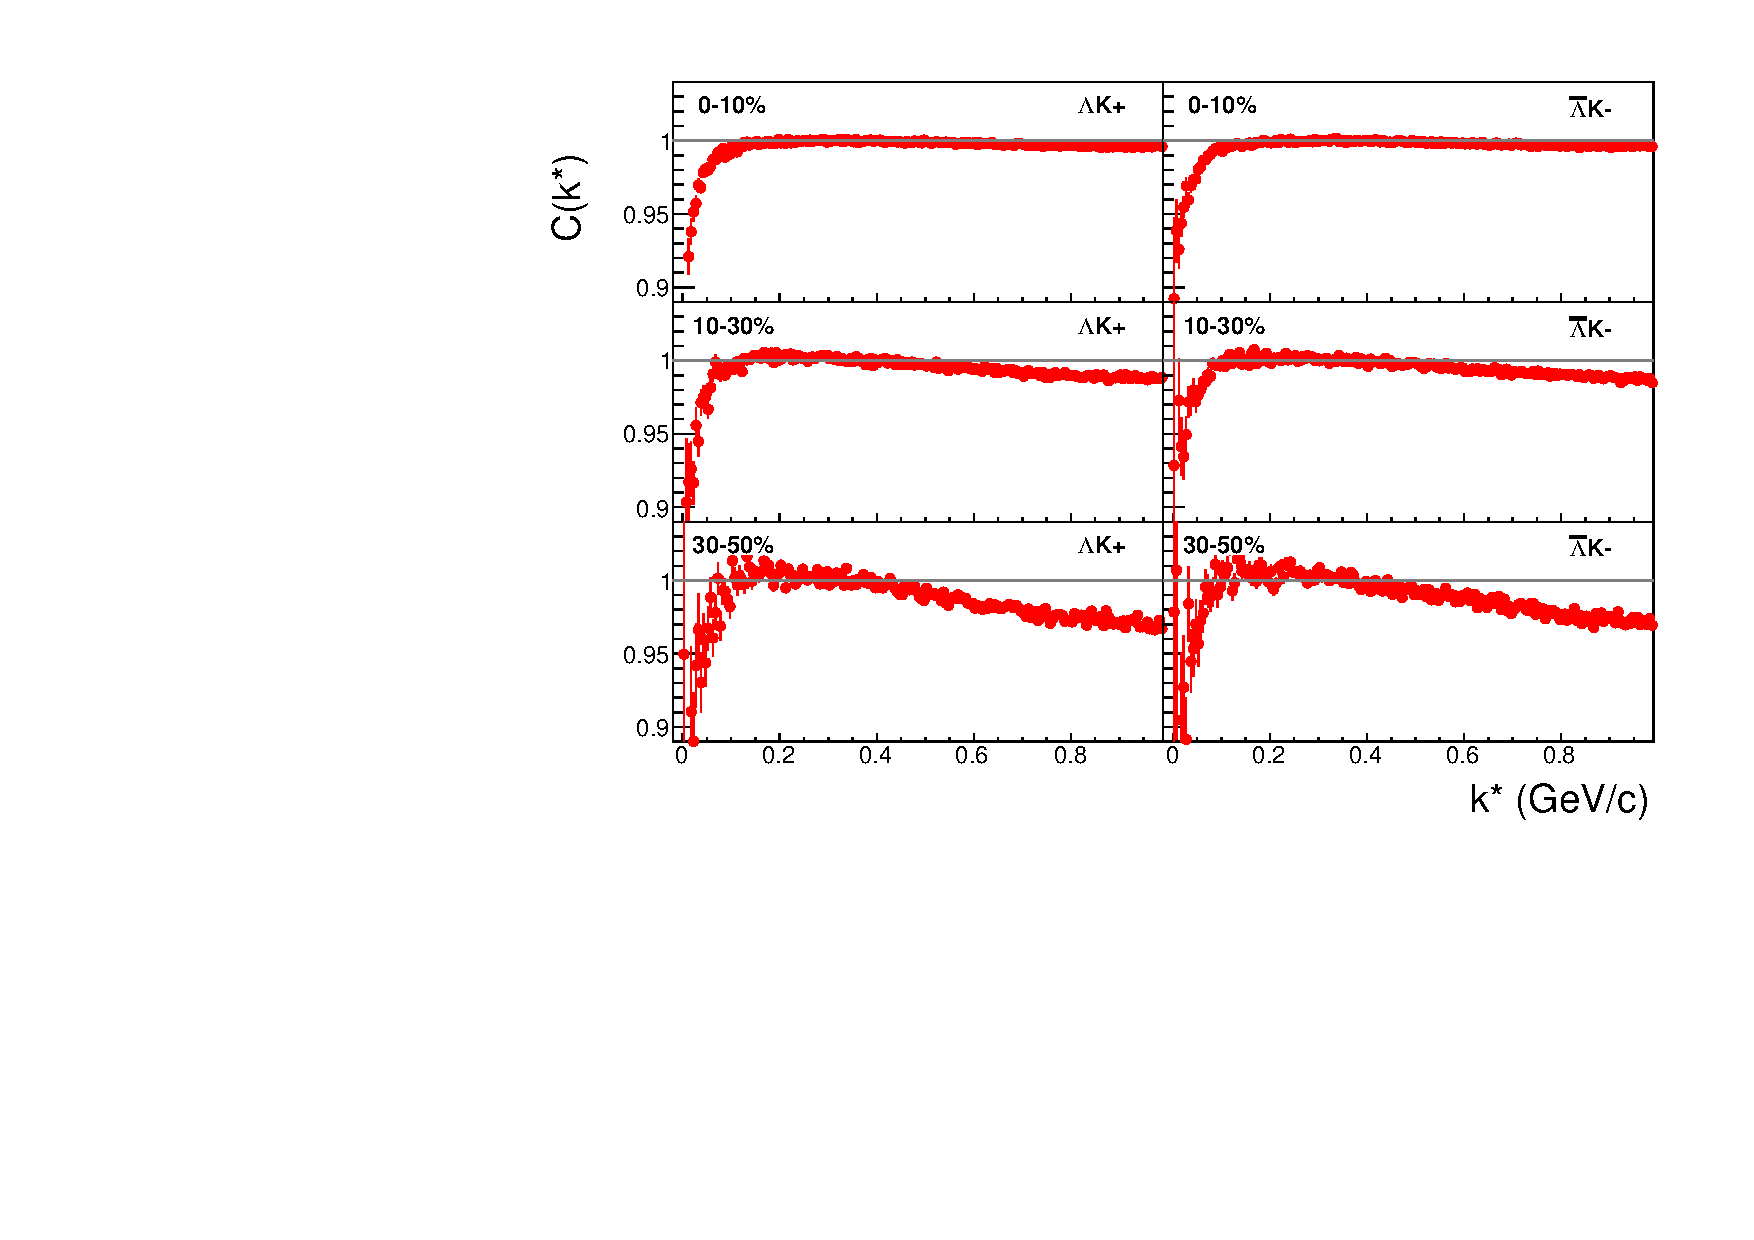
\includegraphics[width=\textwidth]{4_CorrelationFunctions/Figures/canKStarCfsLamKchPwConj.pdf}
  \caption[$\Lambda$K$^{+}$ and $\bar{\Lambda}$K$^{-}$ Correlation Functions]{$\Lambda$K$^{+}$ and $\bar{\Lambda}$K$^{-}$) Correlation Functions}
  \label{fig:LamKchPwConjCfs}
\end{figure}

\begin{figure}[h]
  \centering
  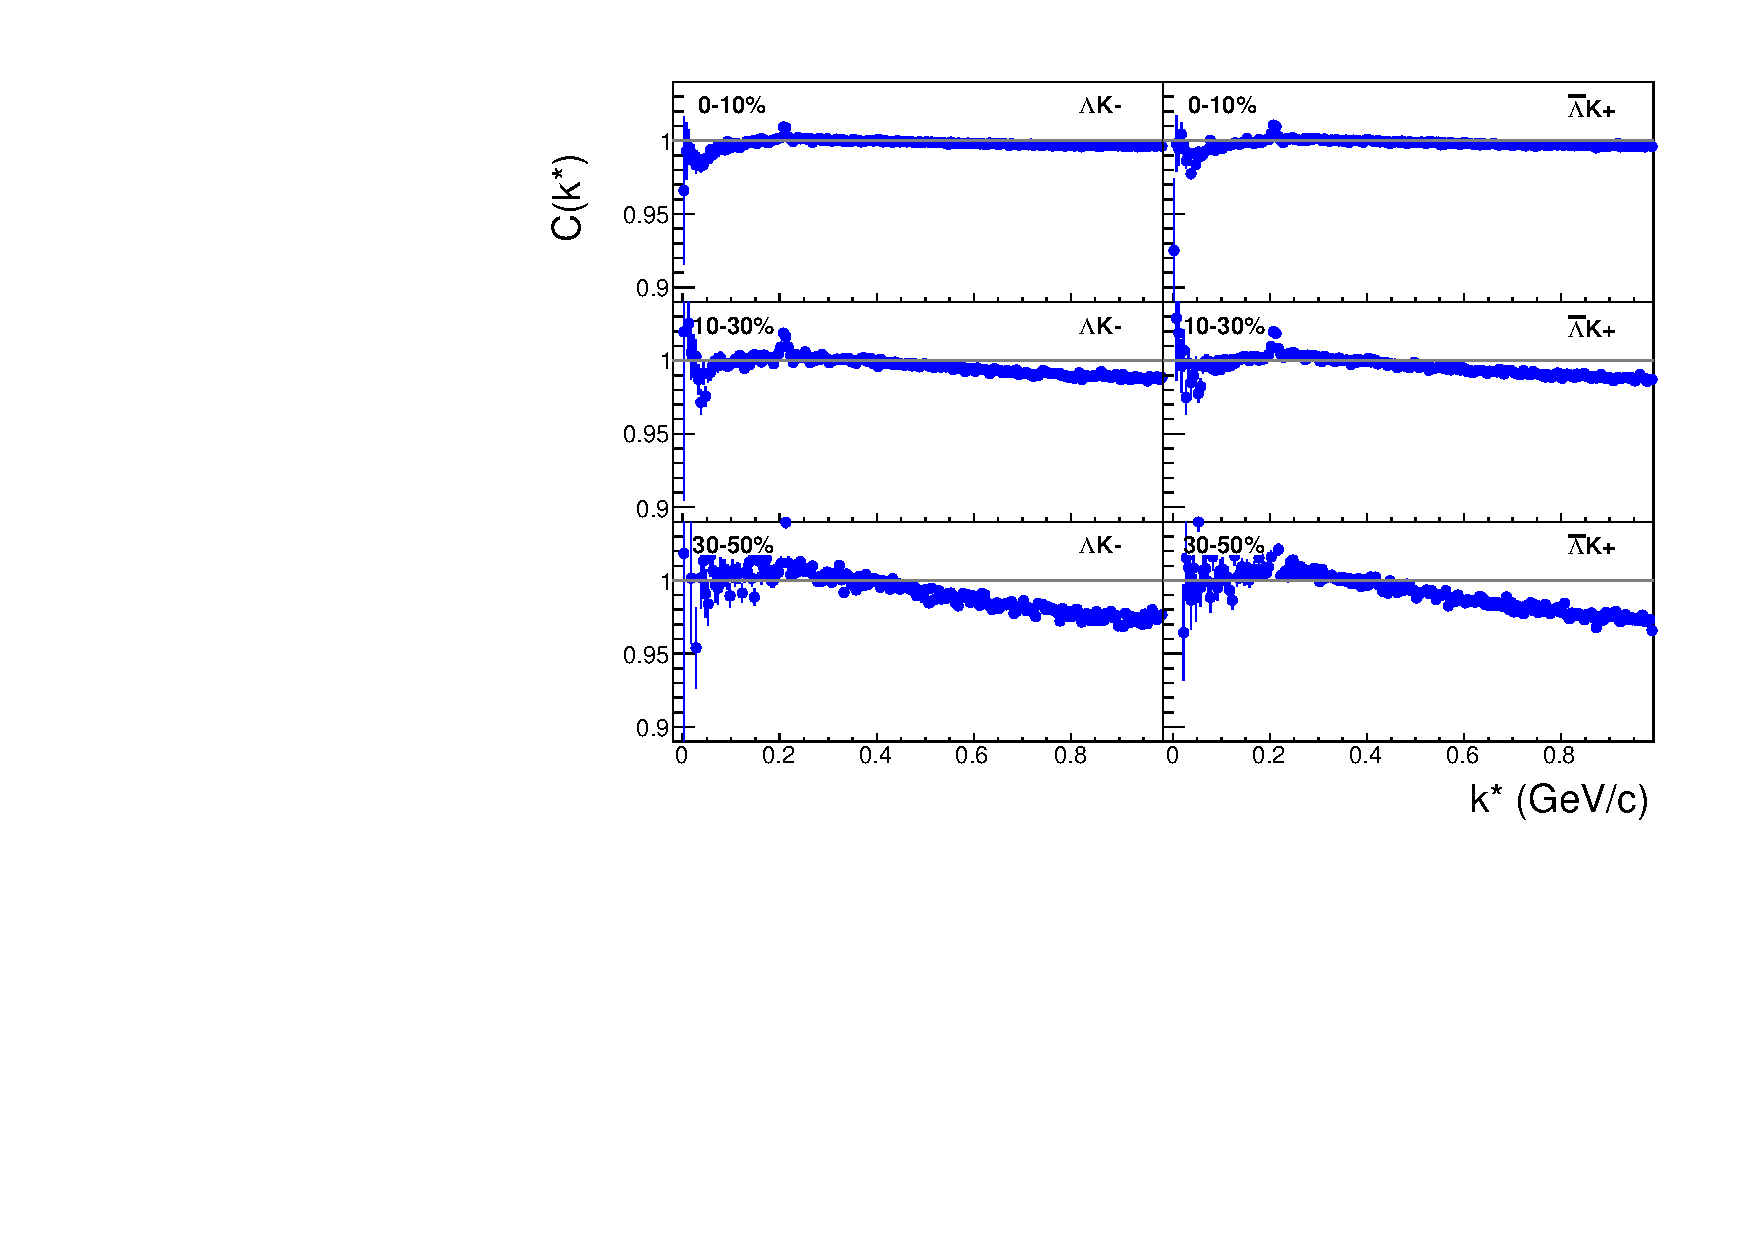
\includegraphics[width=\textwidth]{4_CorrelationFunctions/Figures/canKStarCfsLamKchMwConj.pdf}
  \caption[$\Lambda$K$^{-}$ and $\bar{\Lambda}$K$^{+}$ Correlation Functions]{$\Lambda$K$^{-}$ and $\bar{\Lambda}$K$^{+}$ Correlation Functions) CorrelationFunctions}
  \label{fig:LamKchMwConjCfs}
\end{figure}

\begin{figure}[h]
  \centering
  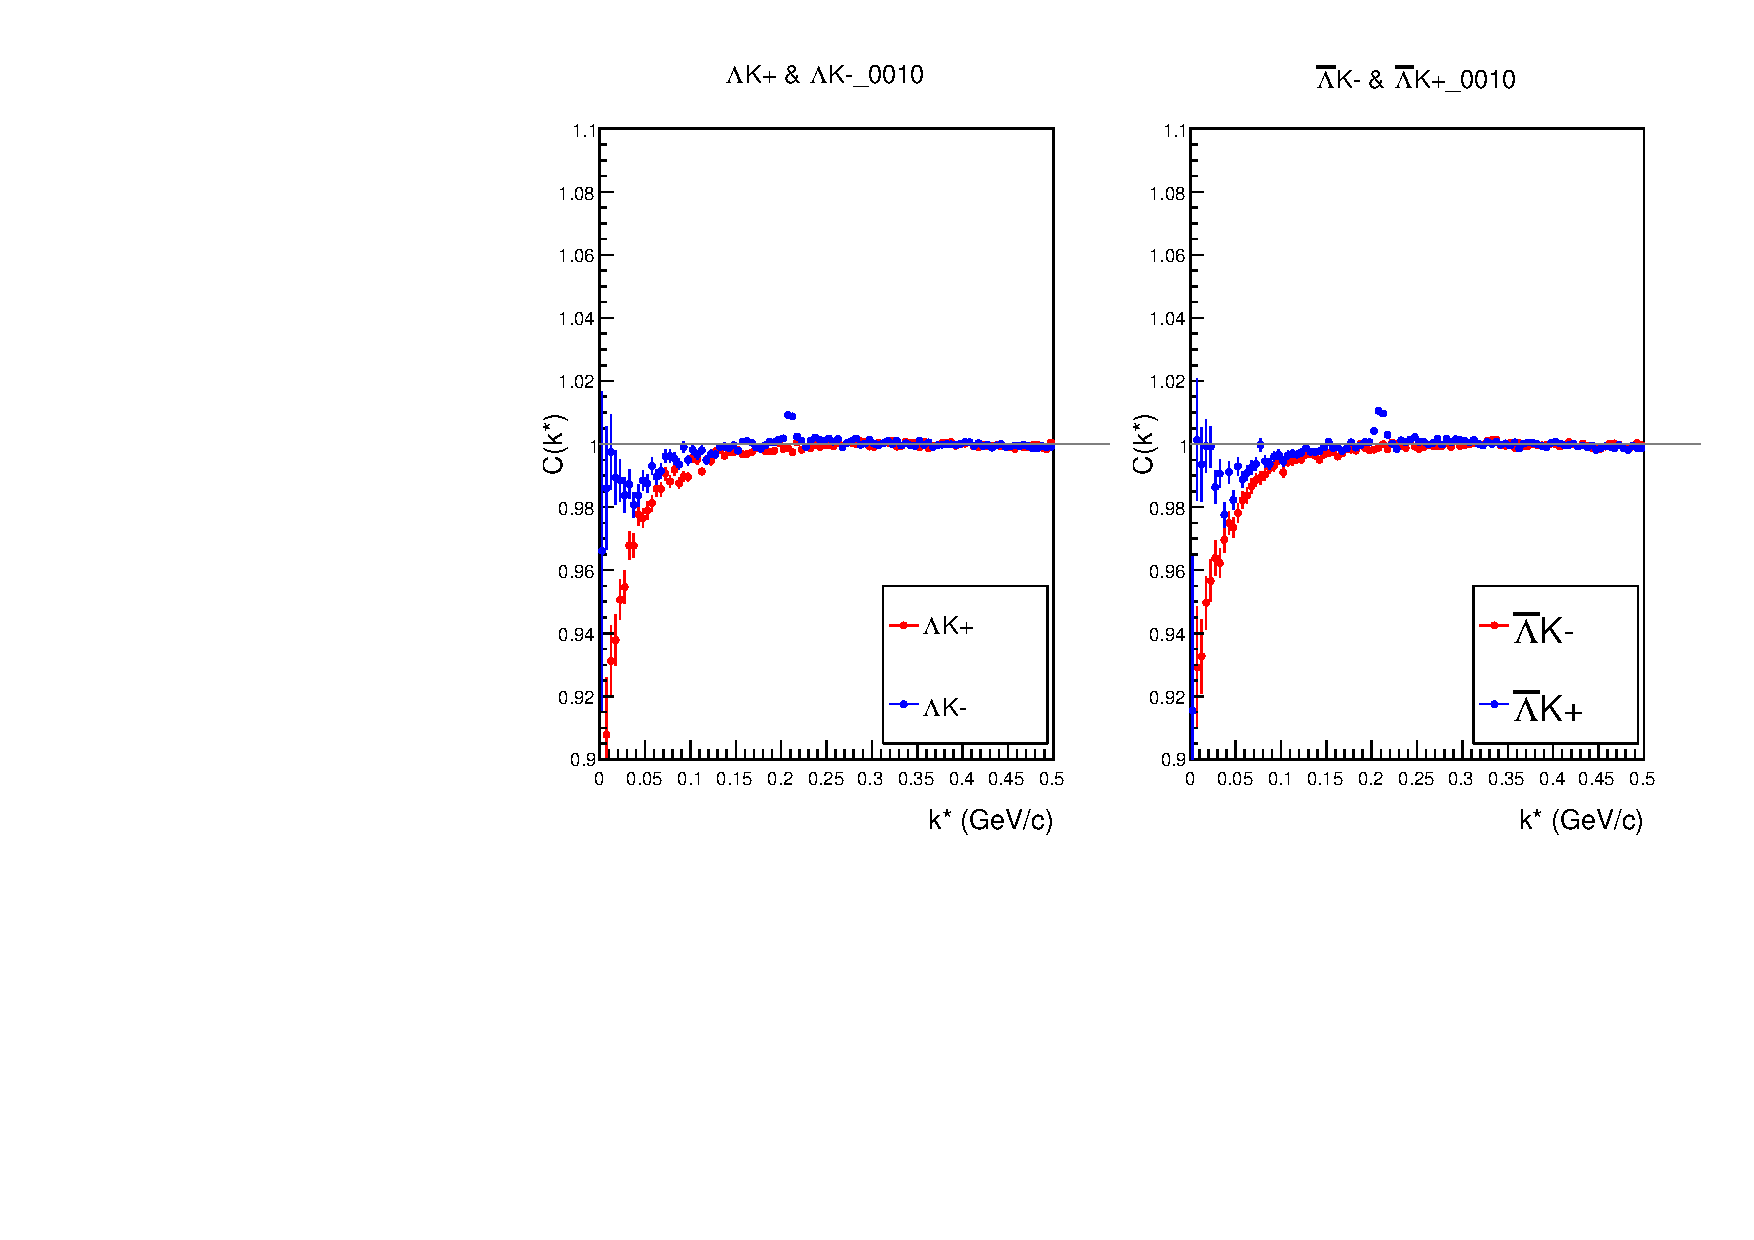
\includegraphics[width=\textwidth]{4_CorrelationFunctions/Figures/canKStarCfLamKchP_0010.pdf}
  \caption[All $\Lambda$($\bar{\Lambda}$)K$^{\pm}$ Correlation Functions]{All $\Lambda$($\bar{\Lambda}$)K$^{\pm}$ Correlation Functions for 0-10\% Centrality}
  \label{fig:cLamcKchCfs0010}
\end{figure}

\end{document}